\documentclass[12pt,letterpaper]{article}
\usepackage[utf8]{inputenx} %Codificacion del texto (ISO Latin1 encoding)

\usepackage{fancyhdr} %Permite acomodar a tu gusto la parte de arriba y
% abajo del documento
\usepackage[spanish]{babel} %Permite definir el idioma del dcumento
\usepackage{graphicx} %Permite exportar imagenes en formato eps
\usepackage{hyperref}
\usepackage{url} %Tipo de fuente para correos y paginas
\usepackage{pgf}
\usepackage{fleqn}
\usepackage{amssymb}
\usepackage{amsmath}
\usepackage{fancyvrb}
\usepackage{makeidx}
\usepackage{multirow}
\usepackage{colortbl} %Permite colocar colores a las tablas
\usepackage{booktabs}
\usepackage[final]{pdfpages}
%%%%%%%%%%
%Margenes%
%%%%%%%%%%
\parskip 1mm %Espacio entre parrafos

\setlength{\topmargin}{0pt}
\topmargin      0.5cm
\oddsidemargin	0.1cm  % Ancho Letter 21,59cm
\evensidemargin 0.5cm  % Alto  Letter 27,81cm
\textwidth	17cm%15.5cm
\textheight	21.0cm
\headsep	4 mm
\parindent	1.2cm
%%%%%%%%%%%%%%%%%%%%%%
%Estilo del documento%
%%%%%%%%%%%%%%%%%%%%%%
\pagestyle{fancyplain}

%%%%%%%%%%%%%%%%%%%%%%%%%%%%%%%%%%%%%%%%%%%
%Fancyheadings. Top y Bottom del documento%
%%%%%%%%%%%%%%%%%%%%%%%%%%%%%%%%%%%%%%%%%%%
% Recuerde que en este documento la portada del documento no posee
% numeracion, pero de igual manera llamaremos a esa primera pagina la numero
% 1, y la que viene la dos. Esto es para tener una idea de las que
% llamaremos pares e impares
\lhead{Modelado de Procesos de Negocio} %Parte superior izquierda
\rhead{\bf \it Departamento de Informática - UTFSM} %Parte superior derecha
\lfoot{} %Parte inferior izquierda. \thepage indica
% el numero de pagina
\cfoot{} %Parte inferior central
\rfoot{\bf \thepage} %Parte inferior derecha
\renewcommand{\footrulewidth}{0.4pt} %Linea de separacion inferior

\newcommand{\primaria}[1]{
	\textbf{\underline{#1}}
}

\newcommand{\foranea}[1]{
	\textbf{\textsl{#1}}
}

\newcommand{\primyfor}[1]{
	\underline{\foranea{#1}}
}

\makeatletter
\newcommand\subsubsubsection{\@startsection {paragraph}{1}{\z@}%
                                   {-3.5ex \@plus -1ex \@minus -.2ex}%
                                   {1.5ex \@plus.2ex}%
                                   {\normalfont\bfseries}}
\newcommand\subsubsubsubsection{\@startsection {subparagraph}{1}{\z@}%
                                   {-3.5ex \@plus -1ex \@minus -.2ex}%
                                   {1.5ex \@plus.2ex}%
                                   {\normalfont\bfseries}}


\makeatother
\makeindex

\begin{document}
\begin{titlepage} 

\title{
\includegraphics[width=120px]{./UTFSM.png}\\[0.5cm] Modelado de Procesos de Negocio \\ \begin{Large}\it Análisis de Natural Response\end{Large}} 
\author{Victor Gonzalez Rodriguez\\\url{victor.gonzalezr@usm.cl} \\
\and Neil Garcia\\\url{neil.garcia@usm.cl}}
\date{\today}
\maketitle
\begin{abstract}
Los procesos de negocios en una empresa, son el motor que permiten a la empresa innovar, crecer y optimizar las áreas en la que la empresa se destaca. Natural Response es una empresa que se ha posicionado a nivel mundial, dentro de las mejores dentro de su rubro, cumpliendo los estándares más exigentes del mercado. Por esta razón, esta empresa se vuelve un interesante objeto de estudio, ya que para cumplir las normas establecidas por los estándares internacionales, debe cumplir procesos muy bien definidos, que permitan sobretodo certificar la calidad de las materias primas y los productos que esta empresa produce. Los procesos más importantes de esta empresa, son los procesos de adquisiciones y de evaluación de proveedores, ya que estos procesos inciden directamente en la calidad del producto que la empresa entregará a sus clientes. Para esto, los procesos se han adaptado a las normas ISO 9000:2000 (calidad de productos), y la norma ISO 9000:2008 (certificación de calidad de los proveedores). El análisis de estos procesos son eficientes, pero sujetos a recomendaciones de mejoras, ya que si bien cumplen las normas, los procesos pueden optimizarse, para así mejorar la producción de la empresa, y así mejorar la posición dominante en el mercado.
\end{abstract}
\end{titlepage}
\newpage
\tableofcontents
\newpage

\section{Introducción}
Natural Response es una empresa joven, la cual se encarga de procesar y exportar productos naturales extraidos sustentablemente de la flora chilena, tales como el árbol del quillay. Esta empresa ha entrado a un mercado que exige altos estándares de calidad, y ha sabido responder a los requisitos comerciales del exigente mercado de las empresas proveedoras de materias primas y de productos procesados a nivel mundial.\\
Actualmente la empresa se encuentra posicionada dentro de las mejores a nivel mundial abarcando cerca del 80\% del mercado mundial, por lo cual es de interés conocer qué procesos de negocio han llevado al éxito a esta joven empresa. Estudiaremos los procesos de adquisición de productos y de la selección de proveedores; estamos hablando de procesos críticos para la empresa, ya que la mayor parte de sus ingresos se deben a exportaciones al extranjero, los cuales exigen estándares de calidad tales como la norma ISO 9000:2008, la cual asegura la calidad de los productos y de los proveedores de sus implementos de producción. Es decir, el área de estudio de este documento es el área de producción y ventas.\\

\section{Actores y Roles}
\begin{itemize}
\item{Jefe de Adquisiciones y Sevicios Generales}
\item{Proveedor}
\item{Gerente General}
\item{Jefe de Area}
\item{Gerente de Administración y Finanzas}
\end{itemize}

\subsection{Estructura Organizacional}
La empresa Natural Response, tiene una estructura jerárquica de responsabilidades, donde existen 7 niveles de responsabilidades, que van desde CEO hasta operario de planta.\\

La estructura además contempla la inclusión horizontal a nivel gerencial de comités y de líderes encargados de asegurar los estándares a los cuales se somete la empresa, tales como la norma ISO 9000:2000 (aseguramiento de la calidad) y ISO 9000:2008 (aseguramiento de la calidad de suministros y proveedores).

\subsubsection{Organigrama de Natural Response}
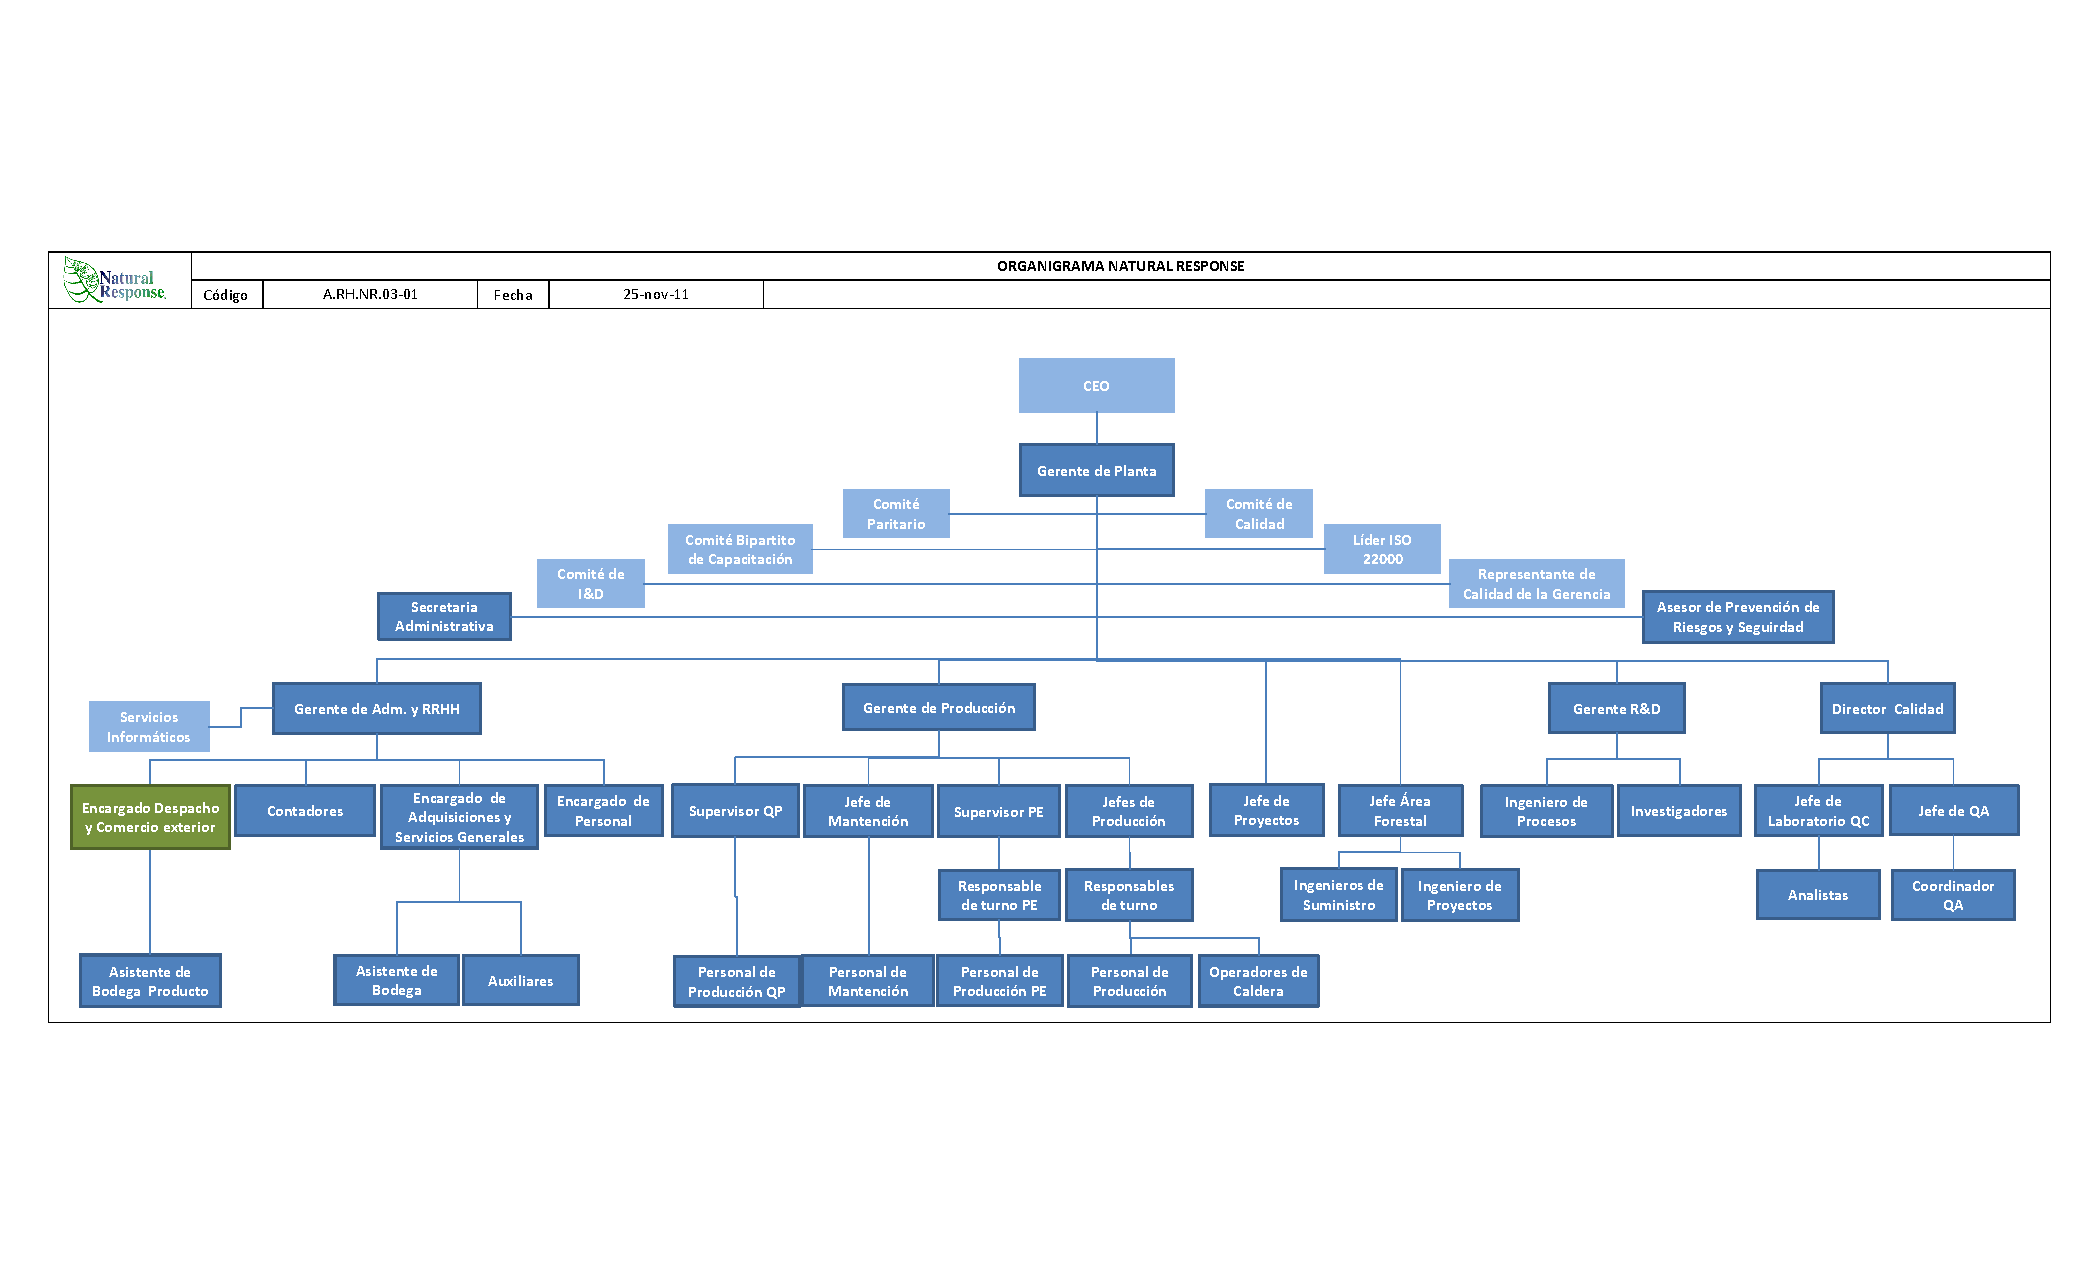
\includegraphics[angle=90,page=1,height=\textheight - 40px]{organigrama_nr.pdf}

\subsection{Especificación de los Actores}

\subsection{Descripción de Roles}

\section{Procesos}

\section{Evaluación e Incorporación de Proveedores}

\subsection{Definición del Proceso}
Natural Response responde a estándares internacionales de calidad, por lo que debe cumplir normas que aseguren la calidad de sus productos y que permitan ser certificados. Es por esto que la evaluación periódica e incorporación de proveedores para Natural Response es sumamente crítico, ya que la empresa necesita certificar la calidad de sus productos, y la norma ISO 9000:2000 les exige certificar la calidad de los proveedores que Natural Response utiliza.\\

Este proceso se aplica a los proveedores de materias primas, insumos y servicios que intervienen directamente en la calidad de los productos o actividades de la empresa. Y el alcance de este proceso llega a la gerencia general, control de calidad y cada área de la empresa solicitante de un insumo, servicio o materia prima incidente en la calidad del producto.

\subsubsection{Actores Involucrados}
\begin{itemize}
\item{Jefe de Adquisiciones y Sevicios Generales}
\item{Proveedor}
\item{Gerente General}
\item{Jefe de Area}
\item{Gerente de Administración y Finanzas}
\end{itemize}

\subsection{Entradas y Salidas}
\begin{itemize}
\item{\textbf{Entrada:} Listado de proveedores ``Provisorios" \footnote{Proveedores a la espera de ser autorizados}}
\item{\textbf{Salida:} Listado de proveedores ``Autorizados'' }
\end{itemize}

\subsection{Indicadores del Proceso}
La empresa utiliza un sistema de evaluación basado en calificación de características ponderadas del proveedor. Esta evaluación se realiza cuando el proveedor se encuentra en estado de ``Provisorio" (entendiendo que es un indicador a priori del proceso), y luego de que ha sido autorizado, despues de un tiempo se procede a evaluar los proveedores en estado de ``Autorizados" (entendiendo que la métrica es a posteriori).\\

Los resultados se evalúan en una escala del 1 al 5, siendo 1 un proveedor muy alejado de las características esperadas, y 5 un proveedor con las características perfectas al perfil de la empresa.

\subsection{Modelo EPC}

\subsection{Recomendaciones}
Se recomienda que la empresa busque nuevas métricas para los indicadores de este proceso, que representen de mejor manera las características que busca la empresa en un proveedor, ya que este punto es crítico para su éxito en el mercado mundial, el cual exige altos estándares de calidad.

\section{Nombre de proceso 2}

\subsection{Definición del Proceso}

\subsubsection{Actores Involucrados}

\subsection{Entradas y Salidas}

\subsection{Indicadores del Proceso}

\subsection{Modelo EPC}

\subsection{Recomendaciones}

\section{Conclusiones}
Los procesos de Natural Response responden correctamente a las normas establecidas por los estándares del mercado, lo cual Natural Response ha sabido aprovechar para tomar una posición dominante del mercado de materias primas extraidas sustentablemente de flora exótica.\\

Además, los procesos llevados a cabo por la empresa, están claramente definidos y sus procedimientos tienen métricas adecuadas y responsables estratégicamente distribuidos, lo cual les ha permitido mantenerse con procesos altamente eficientes, a pesar de que ciertos criterios y métricas podrían ser mejorados, solamente para aumentar el nivel de calidad del producto final.\\

Podemos decir que Natural Response, ha sabido definir sus procesos de negocio críticos para el mercado en el que se desenvuelve, dejandolos en posición dominante del mercado, cumpliendo los altos estándares que sus clientes les exigen para ingresar al mercado internacional.

\subsection{Conclusión de Neil García}

\subsection{Conclusión de Victor Gonzalez}
Me ha tocado ver de cerca la puesta en práctica de estos procesos, y la teoría elaborada acá representa fielmente la práctica de la empresa, lo cual demuestra el alto compromiso con la calidad de sus procesos productivos. Sus procesos productivos son muy eficientes, y es por esto que se han establecido de manera tan firme en el mercado: la calidad de sus productos, la certificación y el aseguramiento de la calidad respaldan la solidez de sus procesos.\\

\section{Recomendaciones}
\textbf{Tecnología.} Es la gran recomendación que se le hace a Natural Response. Ya que si bien los procesos no requieren el uso de tecnologías, es de conocimiento común que las tecnologías mejoran y ayudan a optimizar procesos.\\
Natural Response utiliza el ERP de IBM llamado SAP, el cual entrega una herramientra transversal de trabajo muy eficiente para la gestión de la empresa, pero en las áreas donde los procesos no se ven afectados por este software, se hace necesario métricas y sistemas que apoyen a los procesos. Por ejemplo, para el proceso de evaluación de incorporación de proveedores, se puede utilizar software de soporte para la modelación de problemas multi-criterio, los cuales podrán ayudarlos a entender y predecir de mejor manera cuales son sus mejores opciones.

\section{Referencias}

\end{document} 
